\section{Cross talk measutrements}

Electronic crosstalk is present in both the H12700 and H8500 MAPMTs. This is best observed by plotting the measured charge in one pixel vs. the measured charge in an adjacent pixel. Fig.~\ref{fig:H12700neighbors} and Fig.~\ref{fig:H8500neighbors} show these two dimensional plots for all pixels which neighbor pixel 28 for one H12700 MAPMT and one H8500 MAPMT, respectively. The crosstalk bands are most prominently seen in the pixels directly to the left or right, where the amount of charge collected in one pixel is shown to be proportional to the charge measured in the adjacent one. In particular the bands with a high slope correspond to events where the the pixel plotted on the vertical axis measures some light and the pixel plotted on the horizontal axis has a small amount of charge resulting from electronic crosstalk.


\begin{figure*}
	\centering
	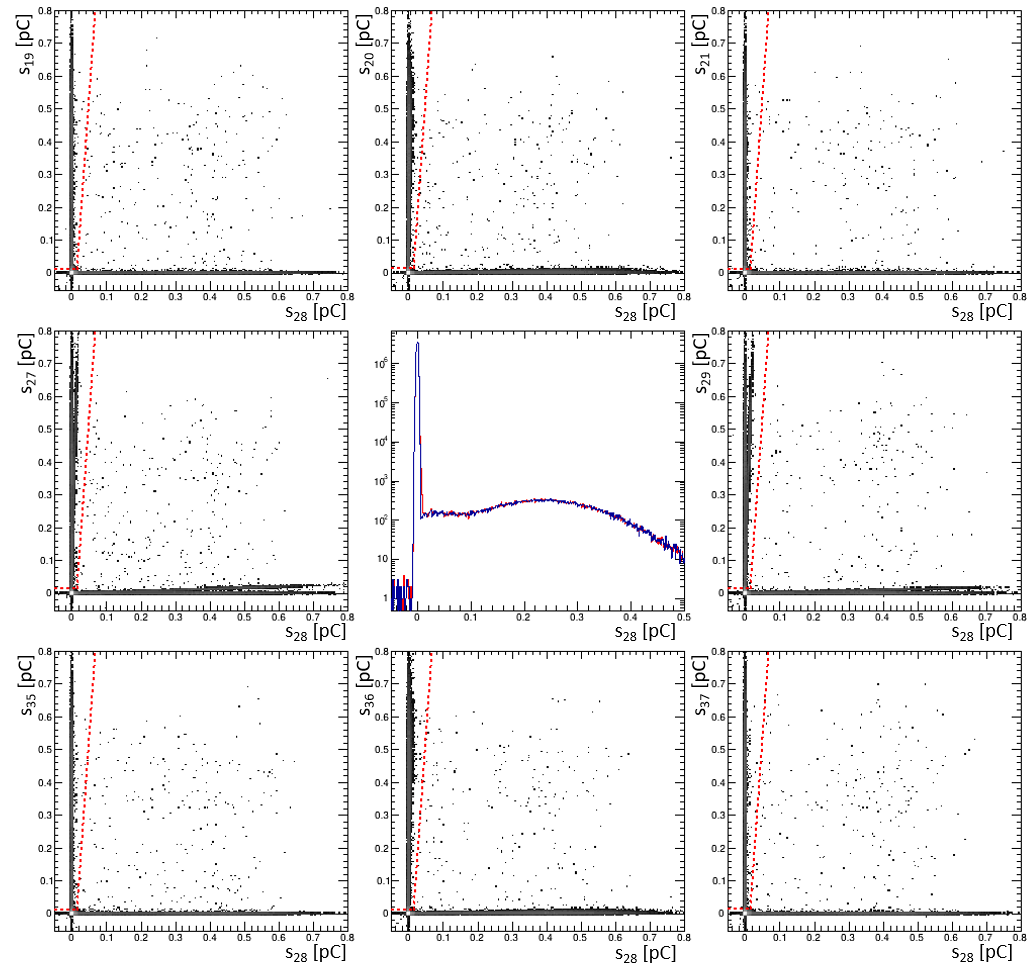
\includegraphics[width=0.95\linewidth]{figures/H12700_ct.png}
	\caption{The charge measured in adjacent pixels is plotted as a function of the charge measured in pixel 28 for a typical H12700 MaPMT. The central plot shows the charge spectrum before (red) and after (blue) removal of the crosstalk events which are cut by the dashed (red) line on the 2-dimenional plots.}
	\label{fig:H12700neighbors}
\end{figure*}
\begin{figure*}
	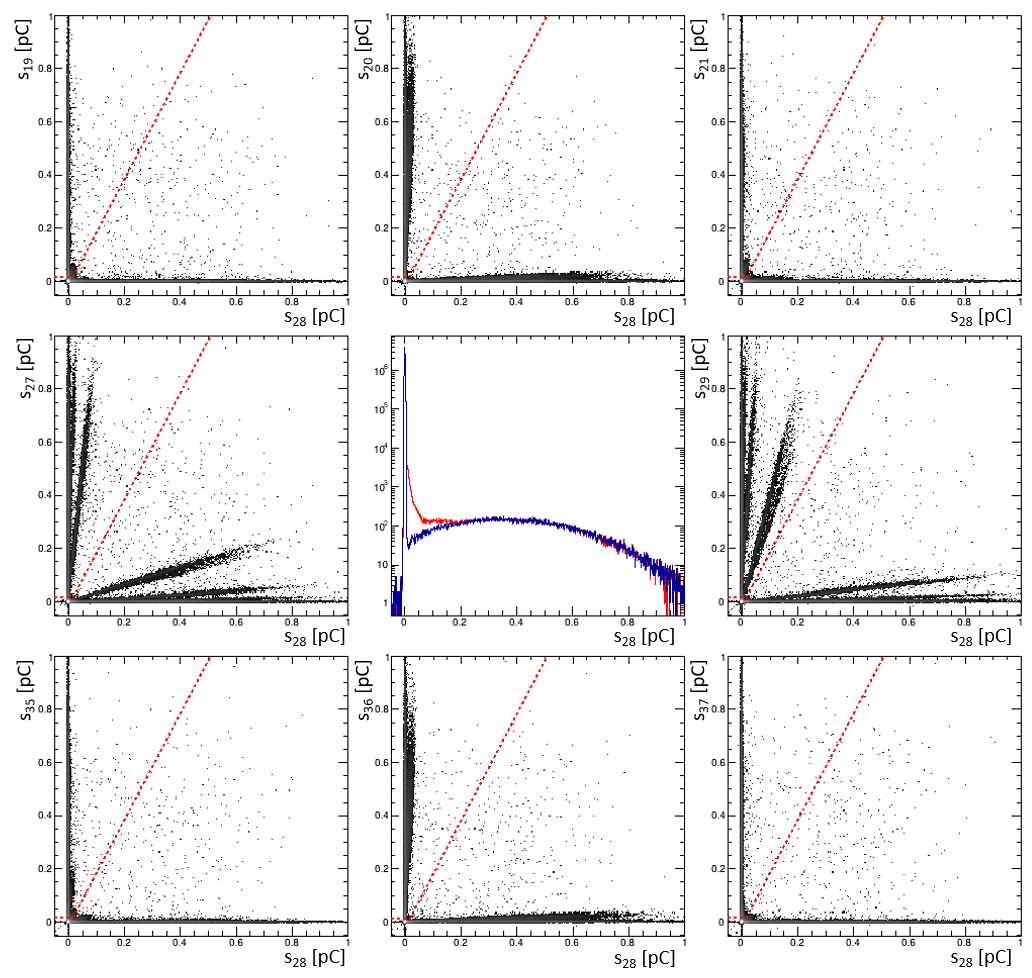
\includegraphics[width=0.95\linewidth]{figures/H8500_ct.png}
	\caption{The charge measured in adjacent pixels is plotted as a function of the charge measured in pixel 28 for a typical H8500 MaPMT. The central plot shows the charge spectrum before (red) and after (blue) removal of the crosstalk events which are cut by the dashed (red) line on the 2-dimenional plots.}
	\label{fig:H8500neighbors}
\end{figure*}


Because the crosstalk events are easily characterized as sloped bands in these two dimensional plots, a simple method was developed to remove the crosstalk offline on an event-by-event basis. For each event the charge collected in a single pixel was compared to the maximum charge collected in the neighboring pixels. This cut is illustrated in Figs.~\ref{fig:H12700neighbors} and~\ref{fig:H8500neighbors} as the dashed (red) line drawn on each 2-dimensional plot. The start of the cut line is placed 7$\sigma$ above the pedestal to avoid removing events belonging to the pedestal distribution. Although the slope of the crosstalk bands can vary between pixels, the slope of the cut line used here is the same for each pixel. The main drawback of this crosstalk cut is that it removes events where adjacent pixels both happen to have a photoelectron emitted from the same laser trigger. However, the fraction of these accidental coincidence events is low when the laser filter is used at the minimal setting. The charge spectra before and after the removal of the crosstalk events in this manner is compared in the central plot in Figs.~\ref{fig:H12700neighbors} and~\ref{fig:H8500neighbors}. For both the H12700 pmt and the H8500 the contribution of the crosstalk to the amplitude spectra appears as a shoulder to the pedestal distribution. However, the relative degree of the crosstalk amplitudes between the two different pmts is quite different. For the H12700 pmts, the crosstalk amplitude is roughly 2-3$\%$ of the amplitude from the pixel where light is incident. In contrast, for the H8500 pmts the ratio of the crosstalk amplitude to the signal amplitude can be as high as 50$\%$ in some pixels. 

As a comparison for the offline crosstalk removal, we collected data where all pixels on the pmt were masked by a black sheet of paper. A 3mm diameter hole was punched over the center of a single pixel to measure the charge spectrum free from crosstalk from the neighboring pixels. 